Bei dem Aufbau des Versuchs wird besonders ein optisches Bauteil hervorgehoben. Die Lummer-Gehrcke-Platte erlaubt eine genaue Auflösung der Spektrallinien. Danach wird die Durchführung des Experiments erklärt.
\subsection{Versuchsaufbau}
Der Versuchsaufbau ist in Abbildung \ref{fig:abb7} dargestellt. Eine mit Cadmium gefüllte Spektrallampe befindet sich in einem Magnetfeld, das durch zwei Spulen erzeugt wird und dessen Magnetfeldstärke veränderbar ist. Der Strahlengang wird durch ein Obektiv und eine Linse fokussiert und mit Hilfe eines Spalts möglichst parallel zur optischen Achse eingestellt. Ein Geradsichtprisma spaltet das emittierte Licht in die Spektrallinien auf. Ein Polarisationsfilter ermöglicht es zwischen $\pi$- und $\sigma$-Übergängen zu unterscheiden. Ein zweiter Spalt dient dazu, eine Spektrallinie auszuwählen. Abermals fokussiert eine Linse den Strahl, damit der Strahl mit einer möglichst geringen Divergenz auf die Lummer-Gehrcke-Platte fällt. Die Lummer-Gercke-Platte (siehe Kapital \ref{sec:platte}) erhöht die Auflösung der Messapperatur. Mit einer Kamera kann das Bild aufgenommen werden, dass durch die Lummer-Gehrcke-Platte entsteht.

\begin{figure}
	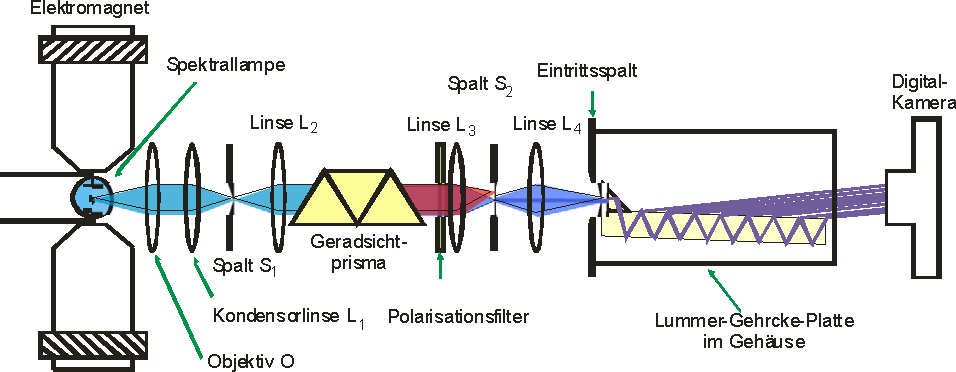
\includegraphics[width = \textwidth]{Abb7.pdf}
	\caption{Versuchsaufbau \cite{\V}}
	\label{fig:abb7}
\end{figure}
\clearpage
\subsubsection{Lummer-Gehrcke-Platte}\label{sec:platte}
Die Lummer-Gehrcke Platte ist eine Glasplatte mit planparallelen Flächen, die durch Totalreflexion an der Innenseite und konstruktive Interferenz der teilweise austretenden Strahlen die Auflösung der Wellenlänge vergrößert (siehe Abb.~\ref{fig:abb8}). Um konstruktive Interferenz zu erhalten muss die Bragg-Bedingung erfüllt sein das heißt, der Gangunterschied zwischen den austretenden Strahlen muss ein ganzzahliges Vielfaches der Wellenlänge sein. Die technischen Daten der in diesem Versuch verwendeten Lummer-Gehrcke-Platte sind:
\begin{align}
	d &= \SI{4}{\milli\meter} \notag \\
	L &= \SI{120}{\milli\meter} \notag
\end{align}
Daraus ergibt sich eine minimale Wellenlängendifferenz, die gerade noch aufgelöst werden kann:
\begin{align}
	\Delta \lambda_D &= \frac{\lambda^2}{2 d} \sqrt{\frac{1}{n^2 - 1}} \\
	\Delta \lambda_{D, \textrm{red}} &= \SI{4.89e-11}{\meter} \notag \\
		\Delta \lambda_{D, \textrm{blue}} &= \SI{2.7e-11}{\meter} \notag
\end{align}
Als Brechungsindex wird für die Rechnung angenommen: 
\begin{align}
n_{\textrm{red}}(\lambda =\SI{644}{\nano\meter}) &= \num{1.4567}  \notag \\
n_{\textrm{blue}}(\lambda = \SI{480}{\nano\meter}) &= \num{1.4635} \quad . \notag
\end{align}
Das Auflösungsvermögen der Lummer-Gehrcke-Platte ist:
\begin{align}
	A(\lambda) &= \frac{L}{\lambda} \left(n^2 -1  \right) \\
	A(\lambda_{\textrm{red}}) &= \num{2.09e5} \notag \\
	A(\lambda_{\textrm{blue}}) &= \num{2.85e5} \notag
\end{align}
Die Lummer-Gehrke Platte erreicht somit eine recht hohe Vergrößerung.
\begin{figure}	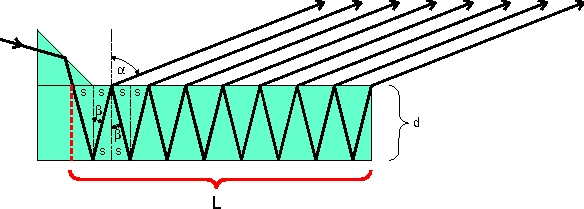
\includegraphics[width = 0.7\textwidth]{Abb8.pdf}
	\caption{Lummer-Gehrcke Platte \cite{\V}}
	\label{fig:abb8}
\end{figure}

\subsection{Durchführung}
Zunächst wird der \textbf{Strahlengang justiert}. Die Linsen werden so verschoben, dass der Strahl gut auf das Prisma, die beiden Spalte und die Lummer-Gehrke-Platte auftrifft. \\
Sobald der Strahlengang gut eingestellt ist, kann das \textbf{Magnetfeld hochgefahren} werden, damit der Zeeman-Effekt eintritt und die Energieniveaus aufspalten. \\
Insgesamt werden fünf \textbf{Bilder aufgenommen}. Für die blaue Spektrallinie macht man ein Foto ohne Magnetfeld, eines mit Magnetfeld und einem Polarisationsfilter in horizontale Richtung und eines mit Magnetfeld und einem Polarisationsfilter in vertikale Richtung. Für die rote Spektrallinie ist das Bild ohne Magnetfeld identisch zu dem Bild mit Magnetfeld und horizontalem Polarisationsfilter, da der $\pi$-Übergang beim normalen Zeeman-Effekt keine Aufspaltung zeigt. Deswegen werden für die rote Spektrallinie nur zwei Bilder benötigt. Für die Bilder mit Magnetfeld wird der Feldstrom, der an der Spule anliegt, jeweils so weit aufgedreht, dass eine Aufspaltung erkennbar ist, die Linien aber nicht verschwimmen. \\
Als letztes wird das \textbf{Magnetfeld kalibriert}. Dazu wird mit einer Hallsonde die Magnetfeldstärke in Abhängigkeit des Feldstroms gemessen. Es ist wichtig sowohl bei ansteigendem als auch bei abfallendem Strom zu messen. So wird die Hysterese-Kurve des Magneten vermessen.